\sloppy
Consideriamo una semplice architettura pipeline a cinque stages, costituita da \textit{instruction fetch IF} $\rightarrow$ \textit{instruction decode e operand assemby ID} $\rightarrow$ \textit{Execute EXE} $\rightarrow$ \textit{Memory Load/Store MEM} $\rightarrow$ \textit{Writeback WB}. Ognuno di questi stages logici ha una mappatura diretta con una macchina cambinatoriale dell'architettura del processore.

\begin{info}
Una macchina combinatoriale (o circuito logico combinatorio) è un sistema logico digitale in cui le uscite dipendono esclusivamente dai valori presenti agli ingressi in un dato istante, senza alcuna memoria degli stati precedenti.
\end{info}

\noindent Diverse fasi di diverse istruzioni, come osservato nel capitolo precedente, possono sovrapporsi nel tempo, e il risultato è un incremento del throughput (istruzioni completate/unità di tempo).
\uppercase{è} immediatamente possibile osservare che il tempo di completamento di un'istruzione (in letteratura \textit{latency}) non migliora, anzi al più peggiora, a causa del già discusso overhead introdotto nel controllo della pipeline (Capitolo \ref{chap:richiami_apc}). Il guadagno in termini di throughput idealmente è pari al numero di stadi, ma nella pratica è limitato dall'overhead di pipeline e dagli \textit{hazards}. 

\begin{warn}
Un \textbf{ciclo di clock} è l'unità di tempo fondamentale dettata dal segnale di clock. Tutte le operazioni elementari avvengono in corrispondenza dei fronti di salita del segnale di clock. Un \textbf{ciclo del processore} è il tempo necessario al processore per completare un'operazione base del set di istruzioni. Nelle architetture RISC un ciclo di processore coincide con pochi cicli di clock. Questo tempo viene misurato in \textbf{IPC} (instruction per clock).
\end{warn}

\noindent Quindi in una pipeline il tempo di attraversamento di un'istruzione è leggermente peggiroato principalmente a causa del fatto che la sequenzialità combinatoriale della macchina viene frammentata da registri che hanno bisogno di un tempo di \textit{setup}. Il parametro che ne beneficia è il clock cycle, che rispetto ad una macchina sequenziale, è ridotto a $\frac{1}{N}$ dove N è il numero di fasi in cui viene frammentata la macchina combinatoriale. In realtà il clock non può essere più veloce del più lento stadio combinatoriale, che ne scandisce un limite superiore. La tecnica della pipeline dunque non è facilmente scalabile: I \textit{path} combinatoriali non possono essere arbitrariamente frammentati; inoltre, superata una certa granularità, gli overhead limitano i benefici. \\ \noindent Nel caso reale, nei diversi stages la latenza è variabile. Questo è dovuto al fatto che l'infrastruttura della memoria è complessa e nel caso peggiore potrebbero verificarsi dei \textit{cache miss}, così come il processore potrebbe avere diverse unità funzionali dedicate all'esecuzione, ognuna con la propria latenza (alcune operazioni sono più lunghe e complesse di altre).

\begin{figure}[ht]
    \centering
    \setlength{\fboxrule}{0.5pt} % spessore sottile
    \setlength{\fboxsep}{0pt}    % senza spazio interno
    \fbox{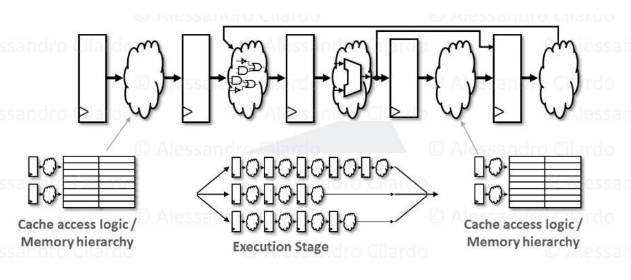
\includegraphics[width=0.6\textwidth]{fig/chapter_2/pipeline_diversity.png}}
\end{figure}

\noindent
Per migliorare l'IPC, si può ricorrere alla moltiplicazione delle istanze di unità funzionali che lavorano in parallelo su più istruzioni. Se l'IPC > 1 si parla di architetture \textbf{superscalari}. \\ \noindent Parlando sempre di pipeline semplice a cinque stadi, possiamo invece agire sull'overhead introdotto dal controllo della pipeline, in particolare risolvere quei conflitti che provocherebbero il blocco (stallo) della pipe. Questo si può fare con l'esecuzione delle istruzioni \textit{out of order}, ovvero con un problema di scheduling vincolato. La pipeline può essere vista nella prospettiva di schedulatore di micro operazioni soggette a vincoli strutturali e dipendenze. I vincoli strutturali sono dettati dell'hardware e scandiscono cosa si può fare in un particolare istante di tempo. I vincoli sulle dipendenze riguardano le relazioni di precedenza tra micro operazioni che devono necessariamente essere soddisfatte nel momento in cui vengono processate dalle unità hardware. 
Rischedulare le micro operazioni può violare i vincoli sulle dipendenze:


\begin{itemize}
    \item \textbf{READ AFTER WRITE (RAW)}: l'operazione di lettura operando di un' istruzione successiva è performata prima dell'operazione di WB sullo stesso registro di un'istruzione precedente;
    \item \textbf{WRITE AFTER WRITE (WAW)}: due istruzioni scrivono lo stesso registro, ma l'ordine di WB è invertito e dunque nel registro si trova un dato vecchio; 
    \item \textbf{WRITE AFTER READ (WAR)}: l'operazione di lettura operando di un'istruzione precedente viene ritardata fino al momento in cui l'operazione di WB di un'istruzione successiva è già avvenuta, distruggendo il contenuto del registro prima che sia letto dall'istruzione precedente.
\end{itemize}

